\chapter{Digital Input and Output with an Arduino}

Overview

In this lab, you'll connect a digital input circuit and a digital output circuit to a microcontroller. Though this is written for the Arduino microcontroller module, the principles apply to any microcontroller.
Table of Contents (hide)

For this lab you will need the following parts:

Solderless breadboard

\begin{figure}[!htb]
 \centering
 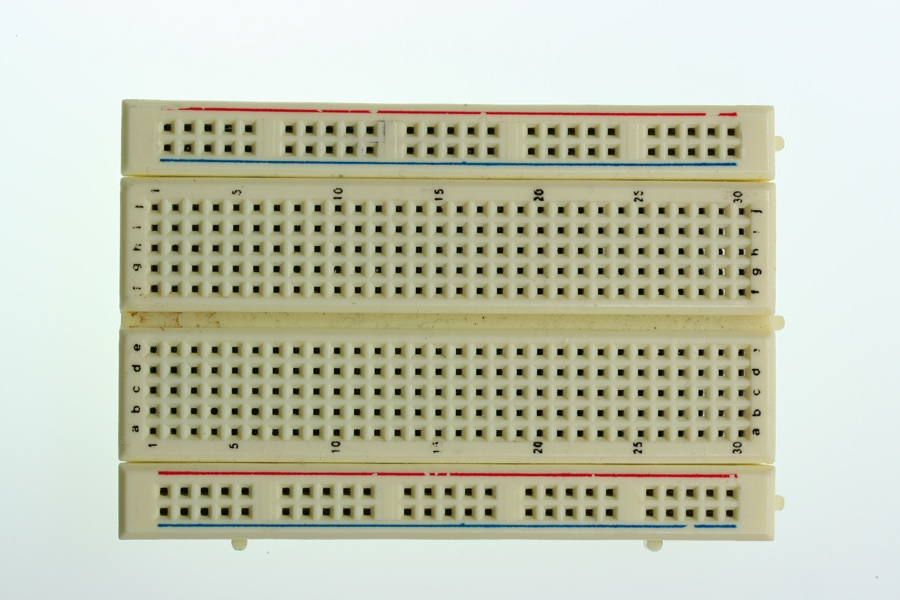
\includegraphics[scale=0.3]{img/digitalio/breadboard.jpg}
 \caption{Solderless breadboard}
 \label{Solderless breadboard}
\end{figure}

22-AWG hookup wire

\begin{figure}[!htb]
 \centering
 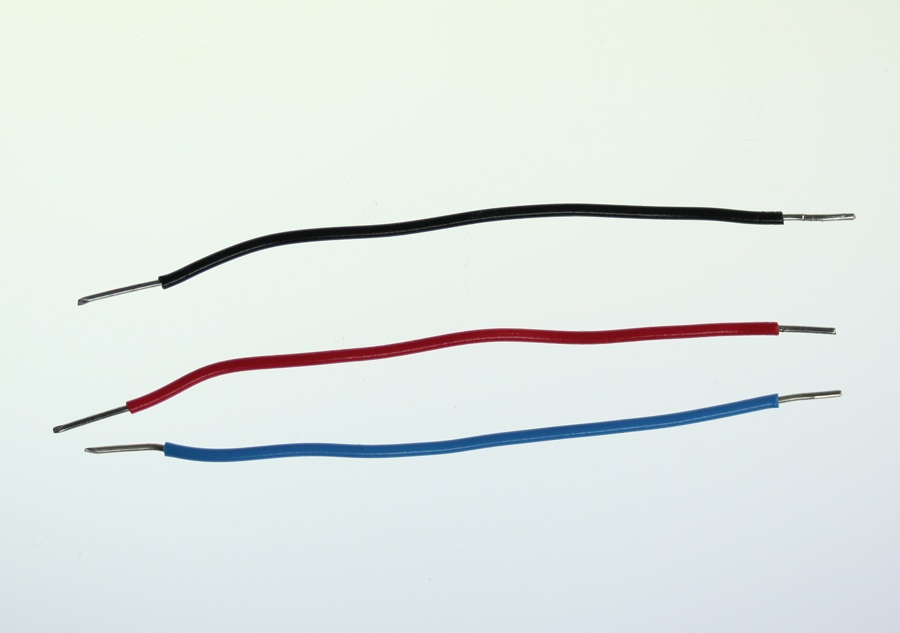
\includegraphics[scale=0.3]{img/digitalio/hookup_wire.jpg}
 \caption{22-AWG hookup wire}
 \label{22-AWG hookup wire}
\end{figure}

Arduino microcontroller module

\begin{figure}[!htb]
 \centering
 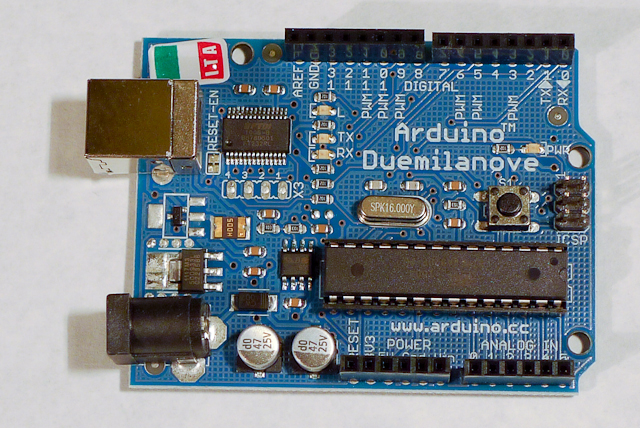
\includegraphics[scale=0.3]{img/digitalio//arduino.jpg}
 \caption{Arduino microcontroller module}
 \label{Arduino microcontroller module}
\end{figure}

Light Emitting Diodes, LEDs

\begin{figure}[!htb]
 \centering
 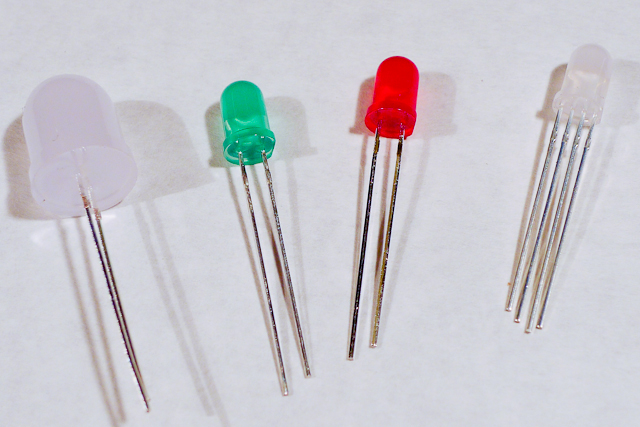
\includegraphics[scale=0.3]{img/digitalio/leds.jpg}
 \caption{Light Emitting Diodes, LEDs}
 \label{Light Emitting Diodes, LEDs}
\end{figure}

220-ohm and 10kilohm resistors

\begin{figure}[!htb]
 \centering
 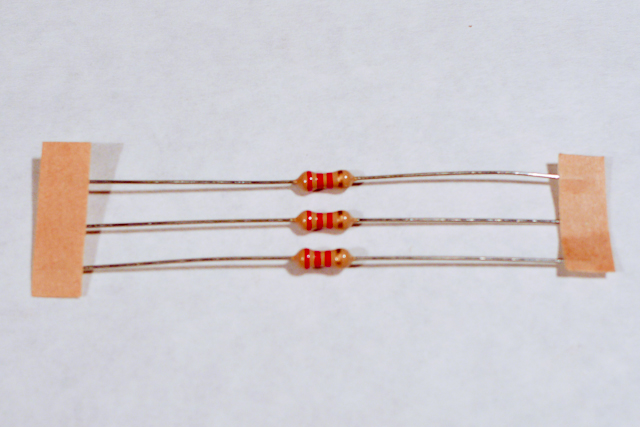
\includegraphics[scale=0.3]{img/digitalio/resistors.jpg}
 \caption{220-ohm and 10kilohm resistors}
 \label{220-ohm and 10kilohm resistors}
\end{figure}


switch or pushbutton

\begin{figure}[!htb]
 \centering
 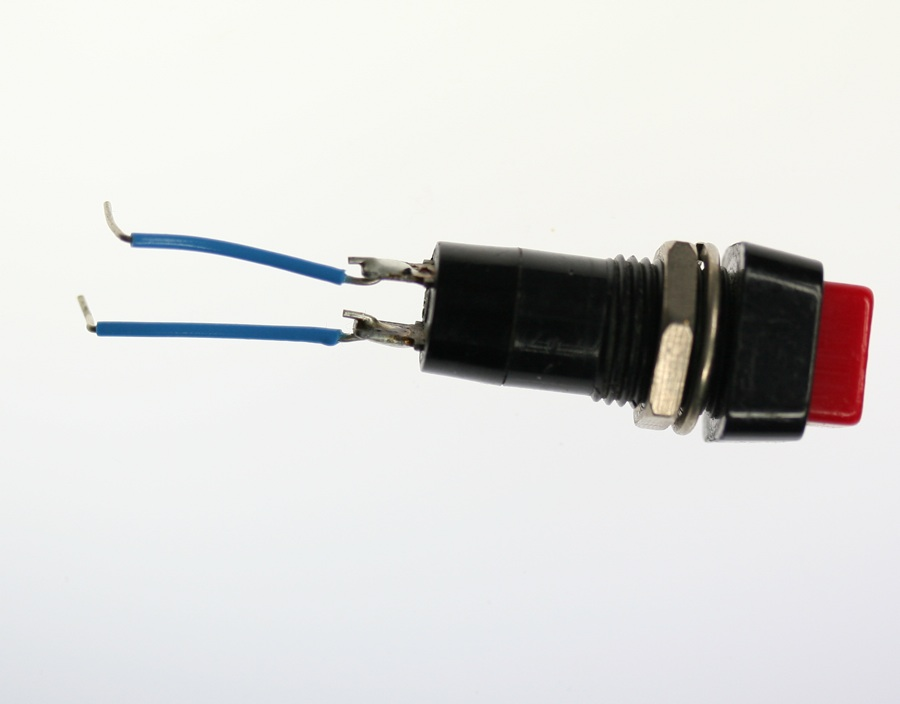
\includegraphics[scale=0.3]{img/digitalio//switch.jpg}
 \caption{switch or pushbutton}
 \label{switch or pushbutton}
\end{figure}

Click on any image for a larger view

\section{Prepare the breadboard}

Connect power and ground on the breadboard to power and ground from the microcontroller. On the Arduino module, use the 5V and any of the ground connections:

\begin{figure}[!htb]
 \centering
 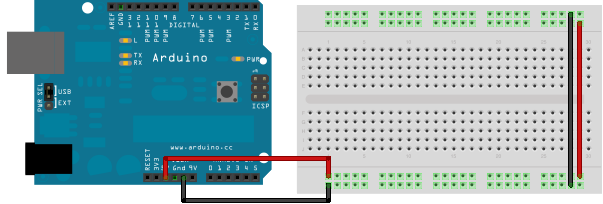
\includegraphics[scale=1]{img/digitalio/arduino_and_breadboard_bb-t.png}
 \caption{arduino and breadboard bb}
 \label{arduino and breadboard bb}
\end{figure}


\section{Add a Digital Input (a switch)}

Connect a switch to digital input 2 on the Arduino. The switch shown below is a store-bought momentary pushbutton, but you can use any switch. Try making your own with a couple of pieces of metal.

\section{Add Digital Outputs (LEDs)}

Connect a 220-ohm resistor and an LED in series to digital pin 3 and another to digital pin 4 of the Arduino.

\begin{figure}[!htb]
 \centering
 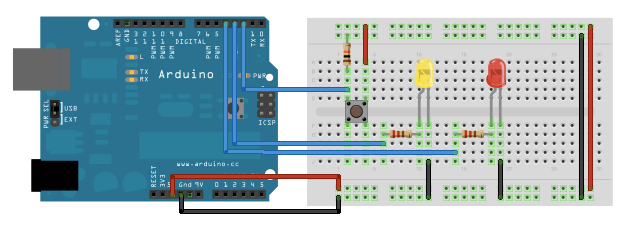
\includegraphics[scale=1]{img/digitalio//digital_IO_lab_bb.png}
 \caption{digital IO lab bb}
 \label{digital IO lab bb}
\end{figure}

\begin{figure}[!htb]
 \centering
 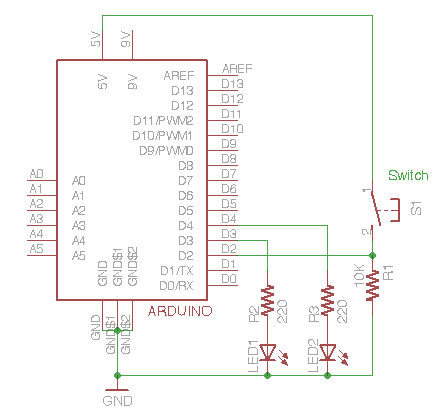
\includegraphics[scale=.6]{img/digitalio/digital_io.png}
 \caption{digital io}
 \label{digital io}
\end{figure}

A note on resistor values: if you don't have a 10-kilohm resistor for the switch, you can use any reasonably high value. 4.7K, 22K, and even 1 Megohm resistors have been tested with this circuit and they work fine. As for the resistor on the LED, the higher the resistor value, the dimmer your LED will be. So 220-ohm resistors give you a nice bright LED, 1-kilohm will make it dimmer, and 10K or higher will likely make it too dim to see.

\section{Program the Arduino}

Connect the microcontroller to your computer via USB. Assuming you've installed the Arduino software environment and the USB-to-serial drivers correctly, you'll find a new serial port in the Tools-->Serial Port menu. in OSX, the name will begin with /dev/tty.usbserial-. In Windows it will start with COM like all the other serial ports.

\begin{figure}[!htb]
 \centering
 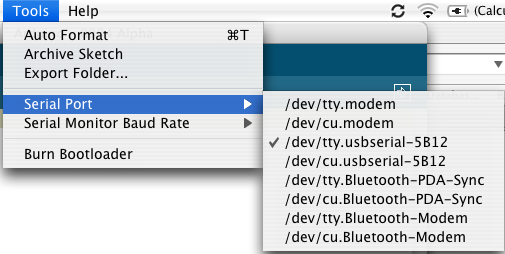
\includegraphics[scale=0.6]{img/digitalio/arduino_tools_menu.png}
 \caption{arduino tools menu}
 \label{arduino tools menu}
\end{figure}

Here's a program that reads the digital input on pin 2. Then it turns on the LED on pin 3 if the input is high (i.e. the switch is on), or turns on the LED on pin 4 is the input is low (the switch is off):

\begin{lstlisting}[language=C]
 // declare variables:
 int switchPin = 2;      //  digital input pin for a switch
 int yellowLedPin = 3;   //  digital output pin for an LED
 int redLedPin = 4;      //  digital output pin for an LED
 int switchState = 0;    // the state of the switch

 void setup() {
   pinMode(switchPin, INPUT);       // set the switch pin to be an input
   pinMode(yellowLedPin, OUTPUT);   // set the yellow LED pin to be an output
   pinMode(redLedPin, OUTPUT);      // set the red LED pin to be an output
 }

 void loop() {
   // read the switch input:
   switchState = digitalRead(switchPin);

   if (switchState == 1) {
     // if the switch is closed:
     digitalWrite(yellowLedPin, HIGH);    // turn on the yellow LED
     digitalWrite(redLedPin, LOW);       // turn off the red LED
   } 
   else {
     // if the switch is open:
     digitalWrite(yellowLedPin, LOW);   // turn off the yellow LED
     digitalWrite(redLedPin, HIGH);     // turn on the red LED
   }
 }
\end{lstlisting}

Click the Verify button to compile this code. Then press the reset button on the Arduino module and click the Upload button to upload the program to the module. After a few seconds, the following message will appear in the message pane to tell you the program was uploaded successfully.
Binary sketch size: 5522 bytes (of a 7168 byte maximum)

Press the switch and watch the LEDs change until you get bored. That's all there is to basic digital input and output!

\section{Get Creative}

This is a suggestion for a possible project. You can do any project you wish as long as it demonstrates your mastery of the lab exercises and good physical interaction.
Many projects can be made with just digital input and output. For example, a combination lock is just a series of switches that have been switched in a particular sequence. Consider the cymbal-playing monkey below:

\begin{figure}[!htb]
 \centering
 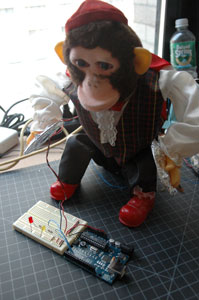
\includegraphics[scale=0.85]{img/digitalio/cymbal_monkey.jpg}
 \caption{cymbal monkey}
 \label{cymbal monkey}
\end{figure}

His cymbals can be turned into a switch by lining them with tin foil and screwing wires to them:

\begin{figure}[!htb]
 \centering
 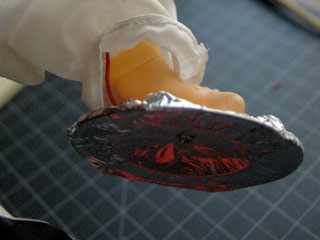
\includegraphics[scale=0.85]{img/digitalio//cymbal_monkey_detail1.jpg}
 \caption{cymbal monkey detail1}
 \label{cymbal monkey detail1}
\end{figure}


\begin{figure}[!htb]
 \centering
 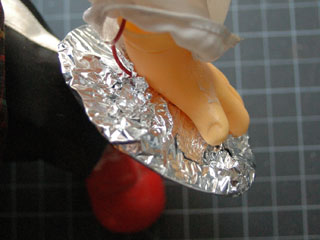
\includegraphics[scale=0.85]{img/digitalio//cymbal_monkey_detail2.jpg}
 \caption{cymbal monkey detail2}
 \label{cymbal monkey detail2}
\end{figure}

Those wires can be run to a breadboard and used as a switch. Then the microcontroller could be programmed to listen for pattern of cymbal crashes, and if it sees that pattern, to open a lock by switching on a digital output.

Come up with your own physical interface for a combination lock.

